\documentclass[fleqn]{homework}

\student{Stephen Brennan (smb196)}
\course{EECS 477}
\assignment{Homework 5}
\duedate{November 23, 2015}

\usepackage{mathtools}
\usepackage{graphicx}
\usepackage{enumerate}
\usepackage{booktabs}

\begin{document}
  \maketitle

  \begin{problem}{1}
    \begin{question}
      Apply the capacity-scaling algorithm to the minimum cost flow problem in
      the figure.

      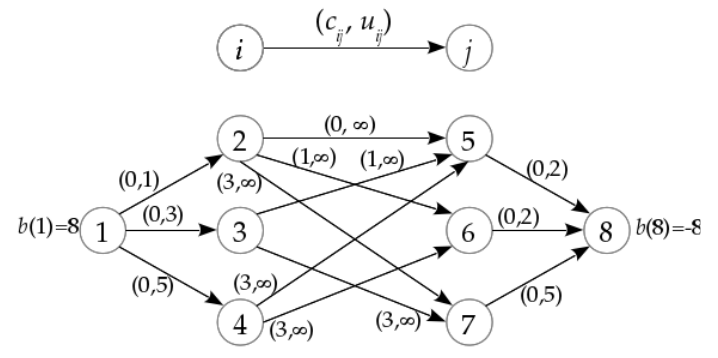
\includegraphics[width=0.6\textwidth]{p1.png}
    \end{question}
  \end{problem}

  \begin{problem}{2}
    \begin{question}
      In this problem, you will revisit the gambling chip game.  Assume that
      there are four chips of value 6, 5, 2, 7, and thus the game ends in two
      rounds.

      \begin{enumerate}[a.]
      \item Write the game in extensive form, and then convert the extensive
        form into strategic form.
      \item Model the strategic form game as a linear program and find the
        optimal mixed strategies for the two players.
      \item Assume that Bob uses his optimal mixed strategy.  Describe a
        deterministic strategy that Alice can use to maximize her winnings.
      \item Find an arrangement of at least two rounds for which the optimal
        strategy is deterministic for both players.
      \end{enumerate}
    \end{question}

    \begin{enumerate}[a.]
    \item Below is the extensive form of the game.  The nodes are game states,
      and at each level the left branch represents the player picking up the
      left chip.  Alice moves first, then Bob, then Alice again.  Bob's final
      move is not shown explicitly since he has no choice.  Below each leaf are
      the payoffs of (Alice, Bob).

      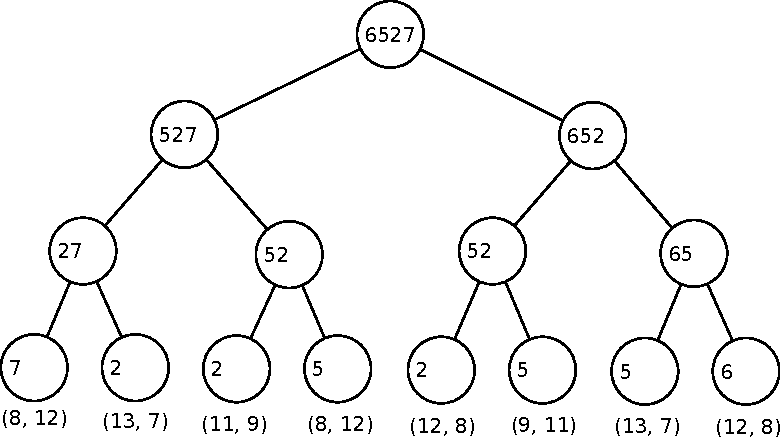
\includegraphics[width=0.6\textwidth]{p2_extensive.pdf}

      In strategic form, we have:

      \begin{align*}
        S^A &= \{(L; L, L), (L; L, R), (L; R, L), (L; R, R), 
                 (R; L, L), (R; L, R), (R; R, L), (R; R, R)\} \\
        S^B &= \{(L, L), (L, R), (R, L), (R, R)\} \\
      \end{align*}

      \begin{itemize}
      \item For Alice, a strategy $(x; y, z)$ represents the following: ``play
        $x$, then if Bob played L, play $y$.  Otherwise, play $z$''.
      \item For Bob, a strategy $(x, y)$ represents: ``if Alice played L, play
        $x$.  Otherwise, play $y$''.
      \end{itemize}

      In order to make this a zero sum game, we will define Alice's payoff as
      her score minus Bob's.  Thus, we can define this table of $H(i,j)$ (which
      we'll need for part b):

      \begin{tabular}{lllll}
        \toprule
        Alice's Strategy & \multicolumn{4}{c}{Bob's Strategy} \\
        \midrule
        & (L, L) & (L, R) & (R, L) & (R, R) \\
        (L; L, L) & $8-12=-4$ & $8-12=-4$ & $11-9=2$  & $11-9=2$  \\
        (L; L, R) & $8-12=-4$ & $8-12=-4$ & $8-12=-4$ & $8-12=-4$ \\
        (L; R, L) & $13-7=6$  & $13-7=6$  & $11-9=2$  & $11-9=2$  \\
        (L; R, R) & $13-7=6$  & $13-7=6$  & $8-12=-4$ & $8-12=-4$ \\
        (R; L, L) & $12-8=4$  & $13-7=6$  & $12-8=4$  & $13-7=6$  \\
        (R; L, R) & $12-8=4$  & $12-8=4$  & $12-8=4$  & $12-8=4$  \\
        (R; R, L) & $9-11=-2$ & $13-7=6$  & $9-11=-2$ & $13-7=6$  \\
        (R; R, R) & $9-11=-2$ & $12-8=4$  & $9-11=-2$ & $12-8=4$  \\
        \bottomrule
      \end{tabular}

    \item In this part, we will refer to the pure strategies of Alice and Bob
      indexed in the order they were presented in part a.  The linear program
      for determining a mixed strategy that maximizes Alice's worst case payoff
      on any of Bob's pure strategies is below:

      \begin{align*}
        \max v &\text{ s.t.} \\
        v + 4x_1 + 4x_2 - 6x_3 - 6x_4 - 4x_5 - 4x_6 + 2x_7 + 2x_8 &\le 0 \\
        v + 4x_1 + 4x_2 - 6x_3 - 6x_4 - 6x_5 - 4x_6 - 6x_7 - 4x_8 &\le 0 \\
        v - 2x_1 + 4x_2 - 2x_3 + 4x_4 - 4x_5 - 4x_6 + 2x_7 + 2x_8 &\le 0 \\
        v - 2x_1 + 4x_2 - 2x_3 + 4x_4 - 6x_5 - 4x_6 - 6x_7 - 4x_8 &\le 0 \\
        x_1 + x_2 + x_3 + x_4 + x_5 + x_6 + x_7 + x_8 &= 1 \\
        x_i &\ge 0, \:\:\:\: i \in [1, 8] \\
      \end{align*}

      The linear program for determining a mixed strategy that maximizes Bob's
      worst case payoff on any of Alice's pure strategies is just the dual of
      the one above, but I will write it below anyway:

      \begin{align*}
        \min w &\text{ s.t.} \\
        w + 4y_1 + 4y_2 - 2y_3 - 2y_4 &\ge 0 \\
        w + 4y_1 + 4y_2 + 4y_3 + 4y_4 &\ge 0 \\
        w - 6y_1 - 6y_2 - 2y_3 - 2y_4 &\ge 0 \\
        w - 6y_1 - 6y_2 + 4y_3 + 4y_4 &\ge 0 \\
        w - 4y_1 - 6y_2 - 4y_3 - 6y_4 &\ge 0 \\
        w - 4y_1 - 4y_2 - 4y_3 - 4y_4 &\ge 0 \\
        w + 2y_1 - 6y_2 + 2y_3 - 6y_4 &\ge 0 \\
        w + 2y_1 - 4y_2 + 2y_3 - 4y_4 &\ge 0 \\
        y_1 + y_2 + y_3 + y_4 &= 1 \\
        y_j &\ge 0, \:\:\:\: j \in [1, 4]
      \end{align*}

      The linear program for Alice is solved in \texttt{p2b\_alice.m}.  Since
      Octave outputs the solution to the dual along with the primal (it is
      called lambda in the output), that is all that is necessary.  Alice's,
      optimal mixed strategy is $\vec{x}^* = (0, 0, 0, 0, 1, 0, 0, 0)$, and
      Bob's optimal mixed strategy is $\vec{y}^* = (0, 0, 1, 0)$.  These achieve
      $v^* = w^* = 4$.  Interestingly, this means that both Alice and Bob's best
      mixed strategies are actually pure strategies: (R; L, R) and (R, L)
      respectively.

    \item Alice may simply use her optimal ``mixed'' strategy found in part b,
      which is the pure strategy (R; L, R).
    \item The given arrangement of chips (6, 5, 2, 7) is such an example.
    \end{enumerate}
  \end{problem}

  \begin{problem}{3}
    \begin{question}
      Consider a data structure implemented as a linked list containing $n$
      distinct items.  The data structure supports the operation
      \texttt{CONTAINS(item)}, which returns true if the list contains the given
      item and false otherwise.  A \texttt{CONTAINS(item)} takes time
      proportional to $O(p)$, where $p$ is the position of the item in the
      list.  Furthermore, once \texttt{CONTAINS(item)} has located the item, it
      can move it forward to any position between the first and the $p$th within
      the $O(p)$ time bound.  In this way, if the same item is being requested
      repeatedly, subsequent \texttt{CONTAINS(item)} will take less time.
      Consider an algorithm for determining whether to move the item forward and
      to which location.

      \begin{enumerate}[a.]
      \item Show that $p \ge n$ in the worst-case for any deterministic
        algorithm.
      \item Use Yao's principle to show that $p \ge (n+1) / 2$ in the worst case
        for any randomized algorithm.
      \end{enumerate}
    \end{question}

    This situation can be represented as a two person zero-sum game, where the
    payoff is the the runtime of the algorithm.  The two players are $A$, the
    algorithm, and $I$, the input.  $A$ tries to minimize the runtime, and $I$
    tries to maximize it.

    \begin{enumerate}[a.]
    \item A deterministic algorithm means that $A$ is using a pure strategy
      (such as ``always move the element to the front'' or ``always move the
      element to $\lfloor p/2 \rfloor$'', etc).  In this case, there is always a
      deterministic strategy that calls \texttt{CONTAINS} on the last item in
      the list each time.  This makes the worst-case payoff $n$ for any
      deterministic strategy of $A$.
    \item For the purpose of this question, we will define the game as a series
      of $n$ rounds ($n$ calls and $n$ executions of the algorithm).  In order
      to determine what the worst-case $p$ would be if $A$ used a randomized
      strategy, we look at the worst-case payoff for this game.  If we think of
      $x$ and $i$ as mixed and pure strategies for $I$ (maximizing player), and
      $y$ and $j$ as mixed and pure strategies for $A$ (minimizing player), then
      the worst-case payoff for the algorithm is:

      \begin{equation*}
        \min_y \max_i H(i,y)
      \end{equation*}

      According to Yao's principle, this follows the inequality:

      \begin{equation*}
        \min_y \max_i H(i,y) \ge \min_j H(x,j) \forall x
      \end{equation*}

      Consider the following mixed strategy $x$: select any ordering of items 1
      through $n$, and call \texttt{CONTAINS} on each one in order.  In this
      case, the optimal strategy $j$ is not to move any element forward in the
      list, because the input will never call \texttt{CONTAINS} on that element
      again.  The payoff of this strategy is:

      \begin{equation*}
        \min_j H(x, j) = \sum_{k=1}^n k = \frac{n(n+1)}{2}
      \end{equation*}

      Since this is over a ``game'' of $n$ calls, the worst-case runtime $p$ for
      a single call to the algorithm is $p \ge \frac{n+1}{2}$.
    \end{enumerate}
  \end{problem}

\end{document}